\chapter{绪论}


\section{研究背景}
人类对外界客观世界的感知信息绝大部分来自视觉,同样,计算机视觉是机器感知世界的基础。计算机视觉技术的发展,是迈向真正人工智能至关重要的一步。

随着互联网技术及数字媒体设备的快速发展,图像、动态图、视频等包含视觉内容的视觉媒体数据呈现指数级增长。例如,截止到2019年3月\footnote{https://expandedramblings.com/index.php/flickr-stats/},图像社区Flickr每日上传图像的记录高达2500万张。截止到2019年10月\footnote{https://merchdope.com/youtube-stats/},视频分享网站YouTube每分钟上传300小时视频数据。海量的视觉媒体数据蕴含丰富的视觉场景,通过对视觉场景进行感知、理解和知识推理,可以帮助人类在日常生活中作出重要的决策,推动社会的发展和进步。

然而,日常媒体数据的视觉场景通常包含大量的物体以及物体间的交互,导致对复杂视觉场景的理解与推理存在巨大挑战。因此,利用计算机视觉技术对海量的复杂视觉场景进行感知和理解,在“大数据时代”的背景下,具有十分重大的意义和应用价值。计算机视觉技术的终极目标就是构建一个计算机模型,使其能够像人一样感知和理解复杂的视觉场景。具体来说,这个模型应该具备以下三种能力:
\begin{asparaenum}
\item 识别和检测视觉场景中所有的组成元素,例如:规则物体(object),不规则物体(stuff),和视觉关系(visual relationship)等;

\item 对视觉场景中感知的视觉信息进行知识推理;

\item 将推理之后得到的知识与人类通过自然语言进行交互。
\end{asparaenum}

总的来说,对复杂视觉场景进行感知和理解主要包含对个体层次的识别、场景层次的识别、理解以及推理等关键技术。本文采取的具体技术路线为逐步感知和理解复杂视觉场景的递进研究,如图~\ref{ch1:fig:scene_understanding}所示,包括物体分类、场景图生成、视觉描述生成、视觉检索与视觉问答:

\begin{figure}[htbp]
    \centering
        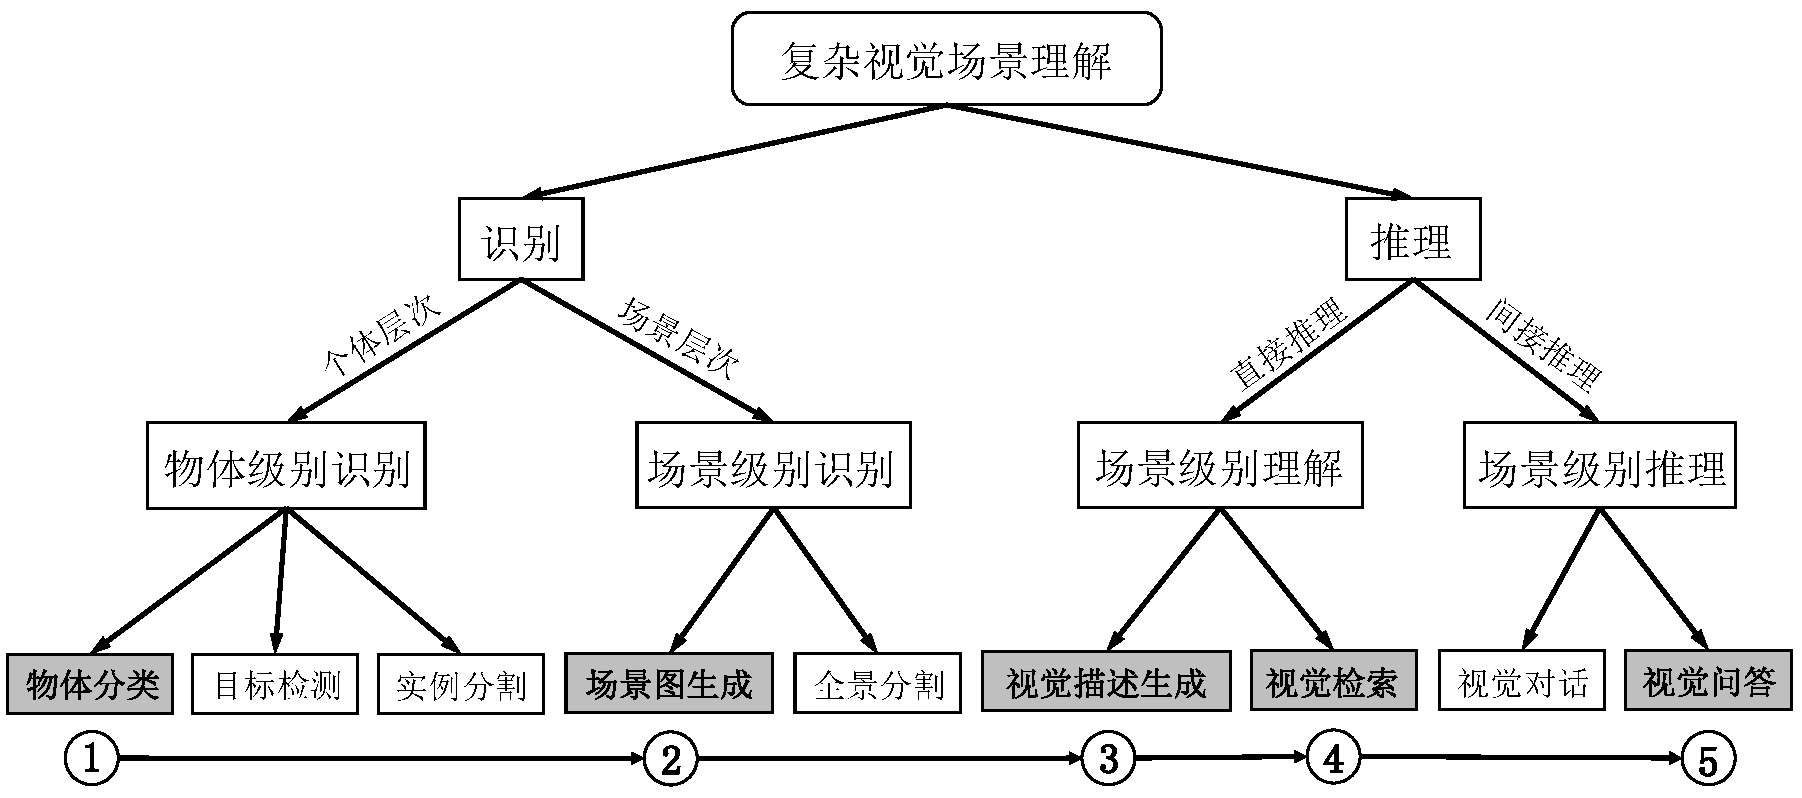
\includegraphics[width=0.95\linewidth]{chapter1/res/scene_understanding.pdf}
    \centering
    \caption{复杂场景感知和理解的关键技术路线}
    \label{ch1:fig:scene_understanding}
\end{figure}

\begin{asparaenum}
\item \textbf{物体识别}:对复杂视觉场景理解的首要步骤是对场景中包含的所有规则物体进行个体层次的识别,它是后续对整个复杂视觉场景进行场景层次的识别、理解和推理的基础。物体识别通常包括其个体的类别(物体分类)、大致位置(目标检测)或者精确位置(实例分割)等任务。具体来说,物体分类~\cite{russakovsky2015imagenet}任务的目标是对物体进行多类别分类,这也是计算机视觉研究中最基本的任务。随着卷积神经网络~\cite{krizhevsky2012imagenet}在大规模图像分类数据集ImageNet上的成功,理想情况下(即每个类别样本数量均衡)的物体分类技术已经日趋成熟,少样本~\cite{fei2006one}或零样本~\cite{lampert2009learning}等更加接近实际应用条件下的物体分类问题已成为近年来的研究热点。目标检测~\cite{ren2015faster}与实例分割~\cite{he2017mask}任务的目标是在物体分类的基础上,同时对物体位置(矩形框或像素)进行定位。通常,这些问题都被转化为多个候选框(或候选形状)的多类别分类和排序问题。本文主要聚焦在零样本条件下的物体分类任务,研究如何保持物体分类所需的属性特征。


\item \textbf{场景识别}:整个视觉场景的识别,除了对所有规则物体进行个体层次识别之外,还需要对物体之间的视觉关系(场景图生成~\cite{johnson2015image})和所有的不规则物体(全景分割~\cite{kirillov2019panoptic})进行识别。对于复杂场景(即场景中存在大量的物体以及物体间的交互),如果忽略了视觉关系或非规则物体,其后续的场景理解和推理的难度将大大增加。对于前者,场景图生成通过对两两物体间的视觉关系进行检测,将非结构化的视觉场景转化成结构化的场景图,简化对整个场景的理解和推理过程。对于后者,全景分割通过对所有非规则物体进行像素级别的分割,实现对整个场景的语义解析。本文主要聚焦在场景图生成任务的研究上,研究如何设计更加鲁棒的优化目标函数。


\item \textbf{场景理解}:在对视觉场景中的所有元素都进行识别之后,计算机模型就可以开始对场景的内容进行理解和推理。对于场景理解而言,一个重要的问题是缺乏统一和标准的衡量指标来判断模型对视觉场景的理解程度。随着递归神经网络(如:LSTM~\cite{hochreiter1997long},GRU~\cite{chung2014empirical}等)在自然语言处理领域(Natural Language Processing, NLP)的成功,在计算机视觉领域开始出现众多视觉与文本融合的多模态研究任务作为场景理解的代理任务,如视觉描述生成~\cite{vinyals2015show}、视觉检索~\cite{gao2017tall}等。对于视觉描述生成而言,模型需要生成描述语句来描述整个视觉场景的内容,并且生成的描述语句是人类能够理解的自然语言。通过对描述语句生成的质量,来判断模型对场景的理解程度。对于视觉检索而言,给定模型一个自然描述语句和一段视频序列,通过对视频序列内容进行理解,从中检索出其视觉场景内容与描述语句一致的视频片段,进而判断模型对场景的理解程度。本文将同时聚焦到视觉描述生成和视觉检索两个任务,研究多模态设定下的视觉场景理解。


\item \textbf{场景推理}:人工智能的最终目标,除了对已经存在的物体进行感知和理解外,还希望像人类一样能够做进一步的场景推理。视觉问答~\cite{antol2015vqa}或视觉对话~\cite{das2017visual}等任务,通常被看作是一种视觉图灵测试,用来判断模型的推理能力。由于测试问题的自由和开放性,理论上一个理想的模型需要具备物体识别、场景识别、空间推理、常识推理等多方面的能力。在理论上,通过对这类问题的求解,可以进一步思考和理解人类对外界世界的感知和推理过程。在实际应用上,可以帮助人类更好的与机器完成互动,推动社会的进步。本文将主要聚焦到视觉问答任务的研究上,研究如何突破近年来视觉问答研究的瓶颈(如:模型受文本偏置影响较大等)。

\end{asparaenum}

\section{研究内容}
本文主要研究如何对复杂视觉场景进行不同层次的感知和理解。

本文分别针对复杂场景理解中上述关键技术进行研究,具体包括以下内容:



\subsection{基于属性保持对抗学习的零样本物体分类}

\subsection{基于反事实多智能体学习的场景图生成}

\subsection{基于通道注意力机制的视觉描述生成}

\subsection{基于密集型自底向上框架的视觉检索}


\subsection{基于反事实样本生成的视觉问答}


\section{本文组织结构}
本文通过对复杂视觉场景理解中的识别、检测和推理,提出了多个新算法。全文共分为八章,后续章节安排如下:
\begin{asparaitem}
\item 第二章介绍了与本文相关的关键技术研究,就零样本物体分类、场景图生成、视觉描述生成、视觉检索和视觉问答等几方面的相关工作和本文的关系进行综述。


\item 第三章介绍了基于属性保持对抗学习的零样本物体分类方法。为了解决零样本物体分类中的属性丢失(semantic loss)问题,本章首次提出图像分类与图像重建本质上是相互冲突的两个子任务\footnote{图像分类需要丢失部分属性特征,而图像重建需要保持所有的属性特征}。算法通过利用对抗学习的思想,对图像分类语义特征与图像重建语义特征进行对抗学习,让图像分类语义特征能够像图像重建语义特征保持尽量多的属性,进而提升零样本物体分类的结果。此项工作发表在国际顶级计算机视觉会议CVPR上.

\item 第四章介绍了基于反事实多智能体学习的场景图生成方法。由于目前绝大多数的图像场景图生成方法都是将所有物体和视觉关系的交叉熵之和作为模型最终的优化目标,这往往忽略了图像中不同物体的重要性。本章首次提出反事实多智能体的训练方法,直接将整个场景图的生成质量当成优化目标,有效地对不同重要性的物体赋予不同的梯度,得到准确的物体和视觉关系分类结果。此项工作发表在国际顶级计算机视觉会议ICCV上。


\item 第五章介绍了基于通道注意力机制的视觉描述生成方法。现有的视觉描述生成的方法往往借助空间注意力机制,让模型在生成不同单词时关注到不同的空间区域。本章首次提出通道注意力机制,通过对图像卷积网络特征的通道维度进行加权,让模型能关注到不同的语义信息。将通道注意力机制和空间注意力机制进行融合,不仅极大地提升了描述语句的生成质量,也加深了人们对卷积网络特征的理解。此项工作发表在国际顶级计算机视觉会议CVPR上。


\item 第六章介绍了基于密集型自底向上框架的视觉检索方法。本章首先对现有的视觉检索两种框架(自顶向下和稀疏型自底向上)进行了分析,首次提出了一种密集型自底向上框架。通过将视频检索序列中的每一帧看成是正样本,极大地增加了训练过程中正样本的数量,解决了自底向上框架下正负样本不均的问题。利用同一帧视频特征对视频序列两端(起始点、终止点)进行预测,也解决了自底向上框架下两端预测相互独立的问题。此项工作发表在国际顶级自然语言处理会议EMNLP上。在密集型自底向上框架的基础上,我们进一步创新,对查询(query)和参考视频(reference video)的交互网络进行设计,提出一种基于图结构的金字塔模型。此项工作发表在国际顶级人工智能会议AAAI上。


\item 第七章介绍了基于反事实样本生成的视觉问答方法。本章首次提出了一种通用的反事实训练样本生成方法,让视觉问答模型能够更加关注图像或者文本中的所有重要内容(如:图像中的区域或问题中的单词)。通过将图像或者文本中重要的区域或者单词替换,同时更改成不同的标准答案,组成新的训练样本。将合成的训练样本和原有的训练样本一起训练,迫使模型关注到被替换的区域或者单词,进而让模型能够关注到正确的视觉区域和问题,提升视觉问答准确率和模型的鲁棒性。此项工作已经投稿至国际顶级计算机视觉大会CVPR上。


\item 第八章对全文介绍的工作进行了总结,并提出了对今后的研究展望。

\end{asparaitem}


\section{本章小结}
本章对复杂视觉场景理解研究进行了叙述,分别介绍了该问题的研究背景、本文主要的研究内容以及全文的组织结构。
